\clearpage
\section{Project Management}
\label{sec:technical}

\subsection{Risk Assessment}

\begin{table}[htpb]
	\centering
	\begin{tabular}{p{0.28\linewidth}  p{0.14\linewidth}  p{0.12\linewidth}
		 p{0.36\linewidth} }

		\textbf{Risk} &
		\textbf{Likelihood} & \textbf{Severity} &
		\textbf{Mitigation Technique} \\ \midrule

	    Part delivery is much
		slower, pushing back
		testing and deadlines &
		Very likely & Medium & % Likelihod + Severity
		Continue to create and iterate on plans more often, test more parts of
		the aircraft more often and with higher frequency. Book training
		grounds more often, and create more precise deadlines with contingency
		in mind. \\ \midrule

	    Pilot failure during competition &
		Likely & High & % Likelihod + Severity
		Maximize opportunities for pilot training, ensure proper mechanisms for
		communication between pilots and other ground crew, and ensure proper
		briefing before flight. \\ \midrule

	    Weather conditions render our aircraft or ground station inoperable &
		Unlikely & Very high & % Likelihod + Severity
		While designing and developing the aircraft, ensure testing in
		unfavourable conditions for the aircraft, and providing pilots proper
		briefing for flight conditions. \\ \midrule

	\end{tabular}
\end{table}

\subsection{Preliminary Schedule and Timelines}

\begin{figure}[h]
	\caption{Competition Timeline}
	\centering
	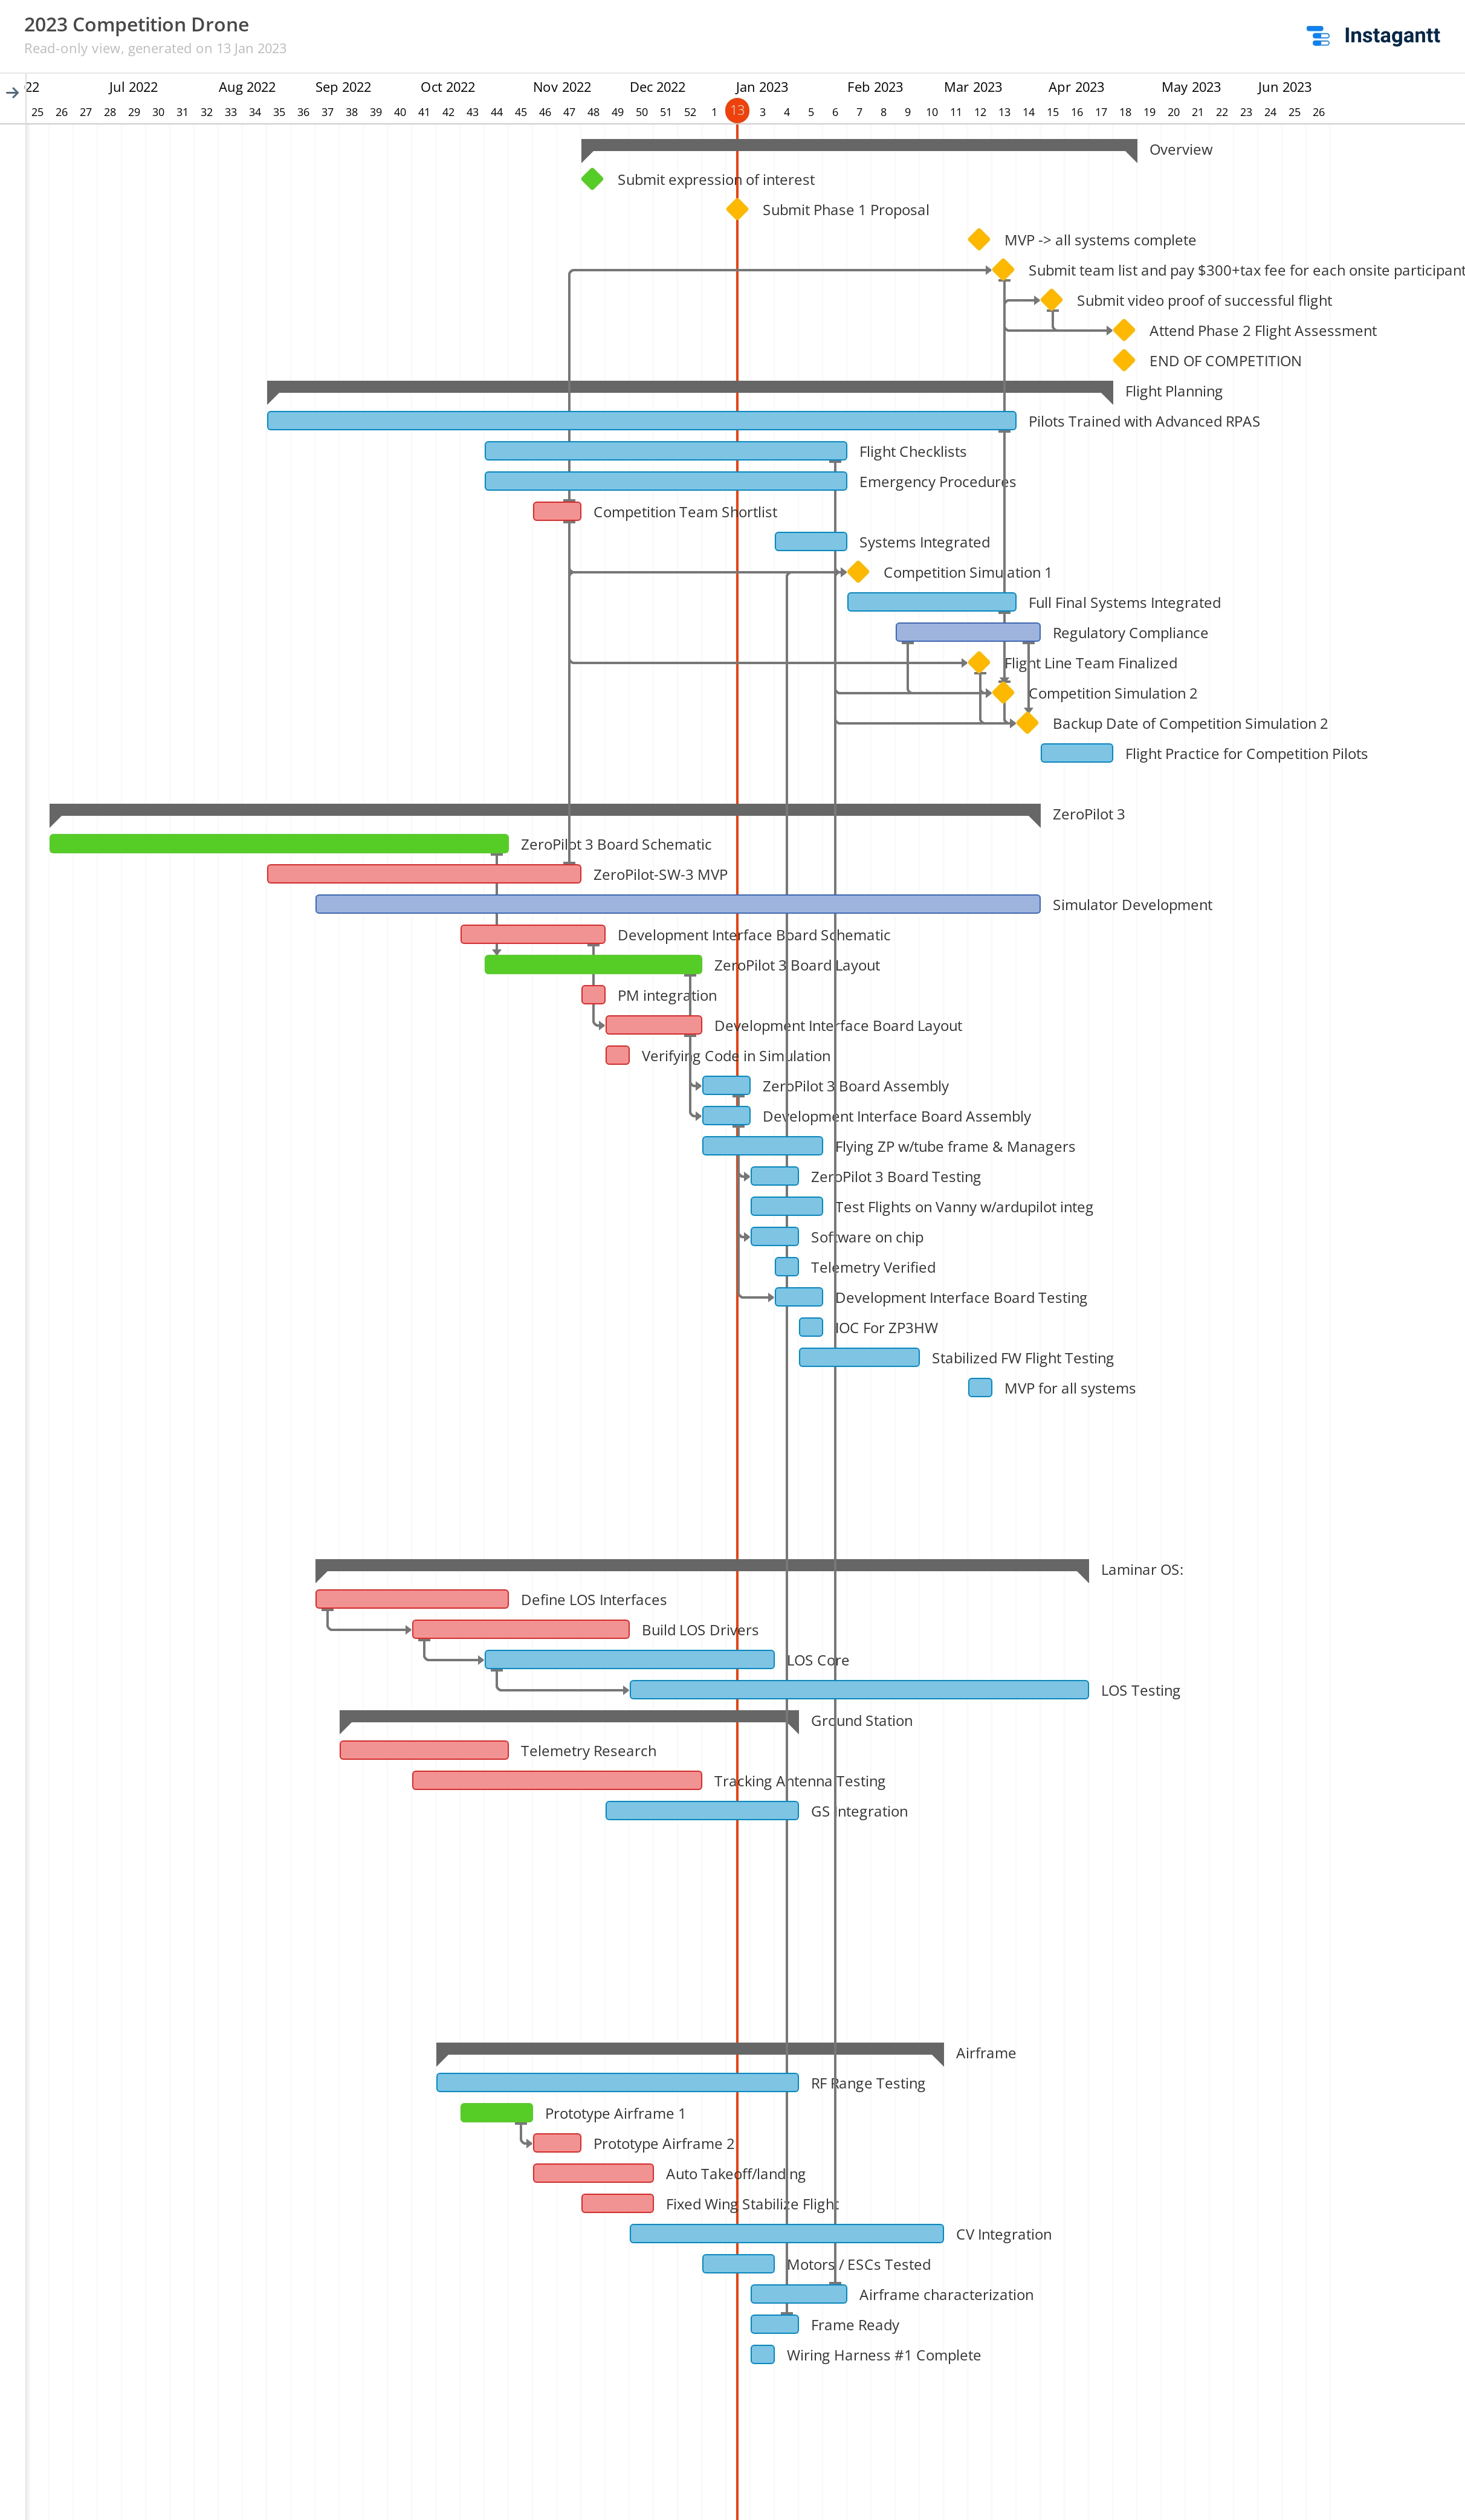
\includegraphics[scale=0.3]{timeline}
\end{figure}


\subsection{Budget}

\todo{Include image of finalized budget chart from Confluence}
